\chapter{Interazioni deboli}

I legami covalenti non bastano per descrivere la complessità delle
strutture molecolari biologiche perché si instaurano forze anche tra
atomi non direttamente legati perché atomi e molecole sono composti da
particelle cariche e si hanno forze elettrostatiche che agiscono anche a
grande distanza.
Il carattere debole delle interazioni rende i sistemi dinamici

\fullpicture*{3_001}{Interazioni forti e interazioni deboli}

Le interazioni deboli rivestono un ruolo importante nei sistemi
biologici, determinando in primis la forma tridimensionale delle
molecole e in più sono importanti anche per l'interazione tra
macromolecole (sia la formazione di complessi sia l'interazione tra
macromolecole e substrati che devono entrare nella macromolecola).

\marginpicture*{3_002}{Interazioni stabilizzanti e non stabilizzanti}

A temperatura ambiente le forze deboli competono con l'energia termica e
quindi le strutture non mantengono la struttura funzionale a qualsiasi
temperatura (denaturazione delle proteine).
Nella denaturazione, non vengono intaccati i legami covalenti ma viene intaccata la
struttura tridimensionale che porta alla perdita della funzionalità.

Le forze deboli contribuiscono alla stabilità del sistema quindi
all'abbassamento dell'energia e quindi sono molto importanti.

\marginbox*{
Le interazioni deboli sono rappresentate dai legami non covalenti e
sono da 1 a 3 ordini di grandezza più deboli dei legami covalenti.
\\Alcuni legami non covalenti tendono a dissociare in uqnto è presente l'agitazione termica delle molecole e in quanto hanno un energhia comparagile a quest'agitazione.
}

\marginpicture*{3_003}{Se ad esempio si usa l’acetilcolinesterasi come enzima, questo ha
una carica positiva sull’azoto che viene attratta dal substrato.\\ Attorno alla carica nel substrato (rosso) si ha un potenziale negativo che attrae l’azoto nel punto preciso dove deve inserirsi.}


\fullpicture*{3_005}{Schema delle interazioni deboli}

\marginbox*{ 
  La perdita di struttura (denaturazione) comporta la perdita di
  funzionalità.
  Se si cambiano le condizioni fisiche si altera la possibilità delle
  proteine di svolgere le loro funzioni
}

Le interazioni deboli sono importanti in chimica biologica perché:
\begin{itemize}
\item
  \emph{Sono facilmente reversibili.} È importante che possano essere superate per rendere dinamico il sistema. Il DNA è stabile ma questo deve essere superato in quanto
  quando il DNA si replica bisogna aprire la doppia elica e rompere i
  legami a idrogeno e questo avviene senza un grande dispendio di
  energia dato che le interazioni sono deboli. Se la molecola fosse rigida, non faciliterebbe le attività cellulari.
\item
  Il \emph{riconoscimento molecolare} avviene mediante l'interplay di molecole
  complementari. La funzione biologica viene raggiunta attraverso
  meccanismi basati sulla complementarietà strutturale determinata da
  interazioni chimiche deboli.
\item
  Le strutture possono formarsi \emph{spontaneamente} e la loro stabilità è
  ristretta ad un intervallo limitato di condizioni ambientali
  (temperatura, acidità, forza ionica, ecc \ldots).
\end{itemize}

Le interazioni considerate sono:
\begin{itemize}
  \item Interazione carica-carica.
  \item Interazione carica-dipolo.
  \item Interazione carica-dipolo indotto.
  \item Interazione dipolo-dipolo indotto.
  \item Forze di dispersione di London.\footnote{Per dispersione si intende un dipolo istantaneo. In media la carica netta è nulla e quindi non c'è dipolo. Però, da un certo istante, la molecola può avere un momento di dipolo da cui deriva un campo elettrico instantaneo}
  \item Repulsione di van der Waals.\footnote{La vicinanza delle molecole comporta che queste si attraggano quando sono distanti, però si respingono qunado sono vicine.}
  \item Legame ad idrogeno.
\end{itemize}

Le interazioni ioniche sono molto importanti nel riconoscimento molecolare. Sono le interazioni più intense.

Nelle forze dipolari, l'energia potenziale dovuta al campo elettrico generato dai momenti di dipolo descresce con $\nicefrac{1}{r^3}$

Nelle interazioni con il dipolo indotto, si vede che l'interazione dipende dalla polarizzabilita della molecola, quindi dalla mobilità degli elettroni

Il campo elettrico $\vec{E}$ può essere dato da una carica o da un dipolo permanente

Le forze di dispersione sono dovute alle rapide fluttuazioni della distribuzione elettronica rispetto ai nuclei. Queste infatti comportano una separazione dei centri di carica elettronica e di carica nucleare, generando un momento di dipolo transiente (o istantaneo). Questo momento di dipolo può indurre un dipolo transiente in un gruppo vicino. Le forze di dispertione quindi consentono una interazione tra un dipolo instantaneo e un dipolo indotto.

Quando due atomi si avvicinano, ci sono delle forze da tenere in considerazione, ovvero una repulsiva e una attrattiva. Di conseguenza l'enegia è data da:
\[
  E = \frac{k_1}{r^{12}}-\frac{k_2}{r^6}
\]
dove il primo termine è quello repulsivo, mentre il secondo termine è il termine attrattivo.

\marginbox{Raggi di van der Waals}{C'è chi dice che il raggio di van der Waals sia la distanza di minima energia e chi invece dice che sia la distanza minima alla quale possono avvicinarsi due atomi.\\
Così come viene definito il raggio di van der Waals, esiste anche un \emph{area di van der Waals} e un \emph{volume di van der Waals}, che rapperentano rispettivamnte le aree e i volumi inpenetrabili di un atomo}

Le forze di van der Waals non sono sempre superiori all'energia termica (a $T$ e $p$ standard). Si ha un'effettiva forza di legame solo quando sono stati coinvolti molti atomi, quindi si può dire che per questo motivo queste forze sono rilevanti quando si ha una complementarietà strutturale, come nell'emoglobina, che è formata da quattro elementi tenuti insieme dalle interazioni deboli.

Un'interazione molto importante è il \emph{legame a idrogeno}. Questo legame ioinvlge atomi elettronegativi, che sono in competizione per lo stesso atomo di idrogeno.

Sono importanti nella stabilità strtturale di proteine e acidi nulceici. Ad esempio, nel DNA, i due filamenti sono tenuti vicini da legami ad idrogeno.

\section{Forze ioniche}

Due cariche possiedono una mutua energia potenziale e si ha quindi
un'interazione coulombiana tra ioni.
L'equazione che regola queste forze è
\[
  F = \frac{q_1 \cdot q_2}{Dr^2}
\]


A distanza corta, queste interazioni sono forti come legami covalenti.

L'energia decresce con 1/r.

Chimicamente significativa fino a 15 \AA{} in proteine.

Un esempio può essere una semplice interazione tra uno ione magnesio e cariche negative presenti sui fosfati (ossigeni nei fosfati) nell'ATP. Il magnesio neutralizza in parte le cariche negative.

\section{Forze dipolari}

Due momenti di dipolo elettrico, $\mu_A$ e $\mu_B$
possiedono una mutua energia potenziale, dovuta al campo elettrico
generato dai momenti stessi.

\marginpicture*{3_006}{Forze dipolari}

Molti aminoacidi hanno dipoli permanenti; questa interazione è meno
forte di quella precedente e dipende da 1/r\textsuperscript{3} e la
forza cala con la distanza molto più velocemente della forza
coulombiana.

In queste interazioni conta anche la geometria perché si hanno prodotti
scalari al numeratore (coseni) e quindi si ha una dipendenza
dall'orientazione relativa delle molecole.
\[
E_d = \varepsilon^{-1} \biggl[\frac{\vec{\mu}_A \cdot \vec{\mu}_B}{r^3} - \frac{3(\vec{\mu}_A \cdot \vec{r})(\vec{\mu}_B \cdot \vec{r})}{r^5} \biggr]
\]

Sono presenti le congiungenti e quindi i baricentri dei dipoli stessi. Ci sono orientazioni che stabilizzano il sistema e interazioni che lo
destabilizzano:

\begin{figure}[H]
  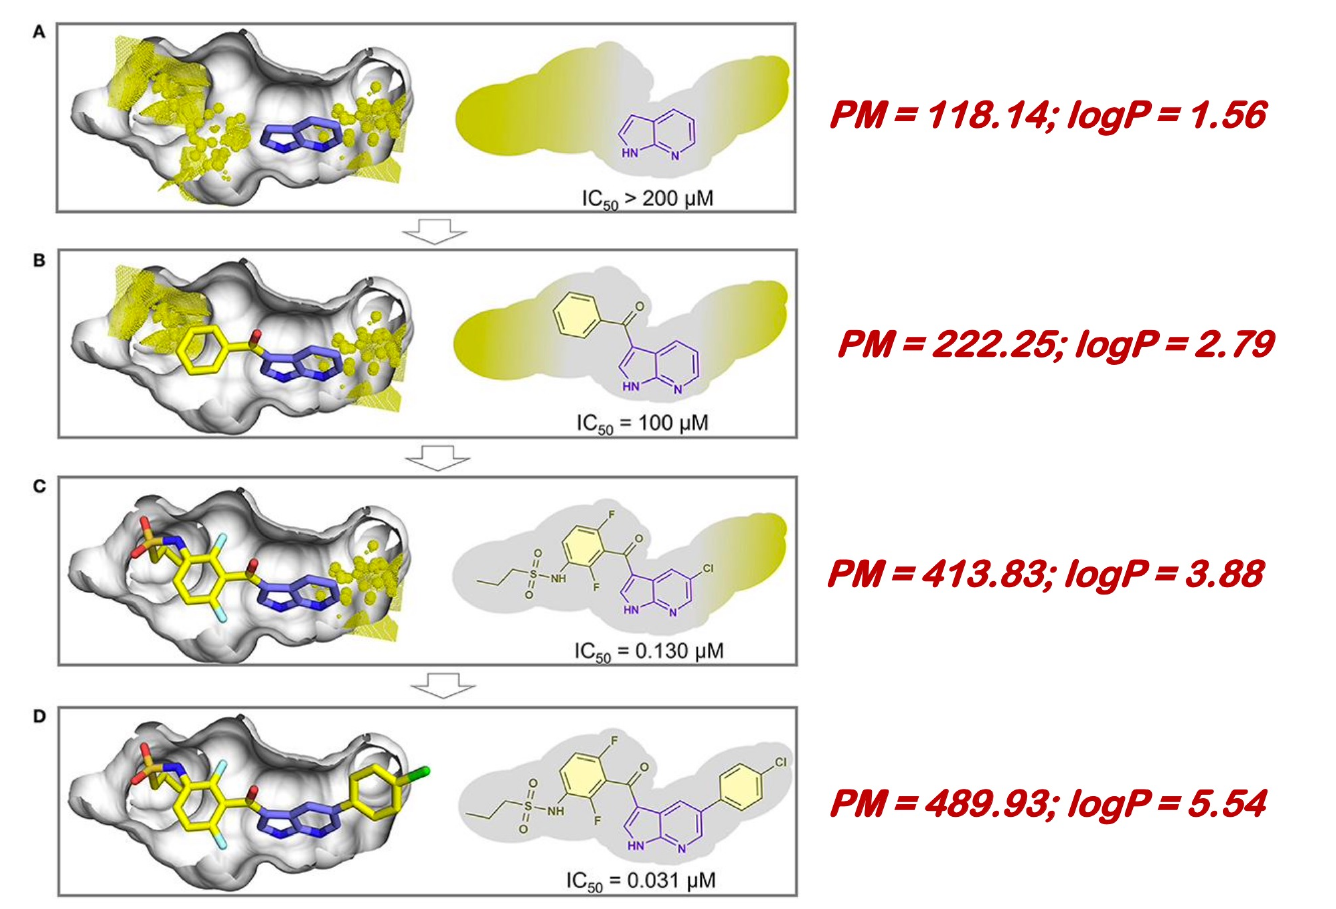
\includegraphics[width=0.5\textwidth]{3_007}
\end{figure}

Quindi, il sistema cerca la struttura con energia minima

\section{Dipolo indotto}

Una molecola soggetta all'influenza di un campo elettrico esterno (E)
subisce un fenomeno di polarizzazione di carica.

\begin{itemize}
\item
  Vengono aumentati i partner delle interazioni possibili.
\end{itemize}

Un elemento è quello che deriva dall'avere la presenza (anche di una
carica) ma comunque di dipolo permanente e quindi un campo elettrico che
circonda un atomo e si suppone che in questo campo elettrico ci sia una
molecola completamente apolare con formazione di un'interazione che è
SEMPRE attrattiva e sempre favorevole.

Gli elettroni in una molecola apolare hanno il baricentro di carica che
corrisponde con quello dei protoni ma questo non è sempre, ma nella
media temporale perché gli elettroni si muovono e istantaneamente
possono essere asimmetricamente posizionati rispetto al baricentro della
carica positiva.

\begin{itemize}
\item
  La presenza del campo elettrico porta gli elettroni a simmetrizzare la
  loro posizione rispetto al baricentro delle cariche positive portando
  ad una polarizzazione della nuvola elettronica che dipende dalla
  polarizzabilità dell'atomo.
\item
  Si crea un momento di dipolo indotto e quindi il campo elettrico
  induce una separazione dei baricentri di carica e porta ad avere
  un'interazione dipolo-dipolo indotto.
\end{itemize}

\fullpicture*{3_008}{Dipolo indotto}

La legge che governa il momento di dipolo indotto è
\[
  \vec{\mu}_{\text{ind}} = \vec{\alpha} \cdot \vec{E}
\]
dove \alpha{} è uguale a\( \alpha = \text{polarizzabilità}\)

Questo tipo di interazioni dipendono dalla forza del dipolo e dalla
polarizzabilità della molecola.

\begin{itemize}
\item
  Non risente del fattore termico
\item
  È a corto raggio (1/r\textsuperscript{5})
\item
  Gli anelli aromatici hanno elevata polarizzabilità
\end{itemize}

\section{Forze di dispersione (London)}

Se si pongono due atomi a una certa distanza senza dipoli o campi
elettrici, questi comunque tendono ad attrarsi e se si avvicinano troppo
o si fondono o si respingono (natura schizofrenica della materia).

Si considera il nucleo con due elettroni e due protoni (He).
In questa configurazione elettronica non c'è momento di dipolo perché i
baricentri coincidono ma se si fanno delle ``foto istantanee'' si vede
che non sempre i baricentri coincidono dato il movimento degli elettroni
con formazione di momenti di dipolo istantanei.

Dire che complessivamente la molecola non è polare vuol dire che
l'integrale temporale è zero (l'orientazione da una parte e dall'altra
annullano i contributi).

La distribuzione degli elettroni rispetto ai nuclei subisce rapide
fluttuazioni che comportano separazione dei centri di carica elettronica
e nucleare, quindi momento di dipolo transiente.

Nel momento in cui si ha il dipolo istantaneo questo va a creare un
campo elettrico che può formare un dipolo indotto in un'altra molecola.
Anche questo tipo di interazione dipende dalla polarizzabilità di
entrambi ma comunque tutti gli atomi hanno questa possibilità di formare
interazione.

\fullpicture*{3_009}{Forze di dispersione}

\marginbox*{
  Si hanno due interazioni attrattive che si formano e nella mediatemporale si ha un'interazione costruttiva.
}

La legge che governa le forze di London è
\[
  V = -\text{C} \cdot \frac{\alpha_1^2 \cdot \alpha_2^2}{R_{12}^6}
\]

L'interazione
è sempre attrattiva quindi si ha sempre un'energia di stabilizzazione ma
questa dipende da R\textsuperscript{6} quindi la distanza deve essere
molto piccola.

\marginpicture*{3_011}{Forze di stacking}

Più è alta la polarizzabilità degli elettroni più è maggiore
l'interazione quindi nel benzene queste sono molto presenti dato che gli
elettroni sono molto polarizzabili.

\fullpicture*{3_012}{
  A seconda del tipo di interazione l'energia associata si sente più o
  meno a seconda della distanza.
}

\subsection{Raggio di van der Waals}

Il raggio di van der Waals determina la
distanza minima alla quale possono
avvicinarsi due atomi. Può essere
considerato approssimativamente come la
distanza alla quale l’energia repulsiva
aumenta rapidamente. L'energia complessiva può essere vista come una somma di due termini, uno repulsivo e uno attrattivo, secondo la legge:
\[
  E_{kl} = \frac{a_{kl}}{r_{kl}^{12}} - \frac{c_{kl}}{r_{kl}^6}
\]
Dove il primo termine è repulsivo, mentre il secondo, attrattivo.

A distanze brevi gli atomi (k,l) tendono ad attrarsi. La distribuzione
degli elettroni rispetto ai nuclei subisce rapide fluttuazioni che
comportano separazione dei centri di carica elettronica e nucleare momento di dipolo transiente.

\fullpicture*{3_013}{Raggi di van der Waals}

Questo dipolo può indurre un dipolo indotto in un gruppo vicino.

La curva di potenziale di Lennard Jones mette in relazione l'energia di
interazione con la distanza tra atomi. Le forze attrattive (rosso) si
respingono con quelle repulsive che dipende da r\textsuperscript{12}
(compenetrazione delle due nuvole elettroniche).

\marginpicture*{3_014}{Intensità delle interazioni di van der Waals}

Il bilancio delle due forze sotto una certa distanza critica va a favore
della forza repulsiva.

Il limite è il raggio di Van der Waals ma la distanza ottimale non
sarebbe quella ma dove si trova il minimo di energia.

Il raggio di Van der Waals determina la distanza minima alla quale possono
avvicinarsi due atomi. Può essere considerato approssimativamente come
la distanza alla quale l'energia repulsiva aumenta rapidamente
(r\textsubscript{VdW}=\sigma).

\marginpicture*{3_015}{Raggi di van der Waals per alcune molecole}

Il raggio di van der Waals definisce il volume impenetrabile di un atomo.
Proprio perché definiscono il volume impenetrabile si possono
rappresentare come un contorno, che è la somma dei r\textsubscript{VdW}
per ogni singolo componente.

Si possono definire un'area (S\textsubscript{VdW}) e un volume
(V\textsubscript{VdW}) che rappresentano aree e volumi impenetrabili.
\[
  S_{\text{VdW} \approx \pi \sigma^2} \qquad V_{\text{VdW} \approx \frac{4}{3} \pi \sigma^3}
\]

\halfpicture*{3_016}{Il raggio di van der Waals viene utilizzato per rappresentare le molecole
nello spazio tridimensionale e quindi è utile per determinare
l'impaccamento di una molecola.}

Le interazioni di van der Waals sono leggermente più forti dell'energia termica a
temperatura ambiente.
Si ha un'effettiva forza di legame solo quando molti atomi sono
coinvolti; questo deternina la complementarietà strutturale.

\paragraph{Complementarietà molecolare}

Oltre alle forze puramente elettrostatiche altre forze deboli
contribuiscono alla complementarietà molecolare.

La complementarietà molecolare dipende da interazioni deboli specifiche
ed è spesso anche di volumi perché le forze vanno in relazione con la
distanza e si cerca di andare più vicino possibile e questo viene
ottimizzato con una complementarietà dei volumi.

\halfpicture*{3_018}{Complementarietà strutturale, con le relative interazioni}

\section{Interazioni di legame a idrogeno}

La natura elettrostatica di queste forze è sottolineata dal fatto che
coinvolgono atomi elettronegativi in competizione per lo stesso atomo di
idrogeno.
È un modo di fare un legame in cui viene messo in comune un idrogeno tra
atomi elettronegativi.

Si ha una carica parzialmente positiva sull'idrogeno e questo legame, tra le
forze deboli, è una forza abbastanza forte ma dipende dai partner.
Le interazioni di legame idrogeno possono essere trattate come
interazioni dipolo-dipolo.
La legge che governa il legame a idrogeno è
\[
  V_{\text{HB}} = - \frac{\text{C}}{R^3_{\text{D-H-A}}}
\]
dove il termine $\text{C}$ è un termine che dipende dalla coppia di atomi che condividono l'atomo di idrogeno 

I partner più comuni sono \ce{N}, \ce{O} e \ce{S} e sono necessari atomi elettron-attrattori con doppietti liberi. La distanza del legame si misura tra
tutti e tre gli atomi.

\marginpicture*{3_019}{Atomi che formano il legame ad idrogeno}

La forza di questo legame dipende molto anche dall'angolazione del
legame stesso.
Si vede quindi che i tre atomi coinvolti sono spesso collineari, quindi a 180° e in questa angolatura si ha la forza maggiore; il legame rimane stabile fino ad un angolo di 150°

\begin{figure}[H]
  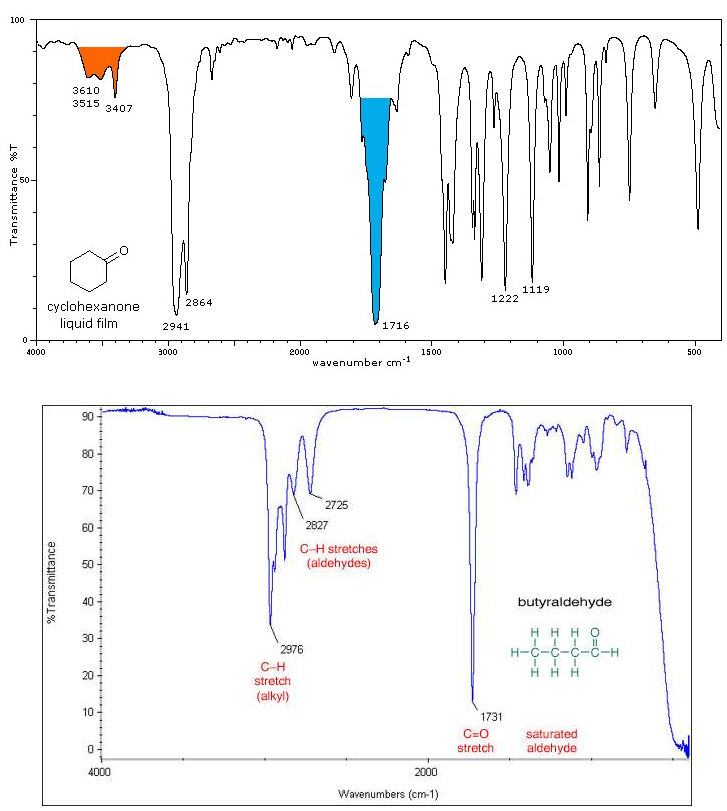
\includegraphics[width=0.5\textwidth]{3_020}
\end{figure}

\marginpicture*{3_021}{Legame a idrogeno forte e debole}

Le strutture secondarie delle proteine (\alpha-elica, \beta-shift) sono basate
sulle interazioni a H, ma sono importanti anche nel DNA.

\marginbox{\alpha-elica}{L'\alpha-elica è una conformazione molto stabile perché è regolare il
termini di legami a idrogeno.\\Questo legame è determinante nella stabilità delle catene considerate
e la sua energia è circa $\nicefrac{1}{20}$ del legame covalente \ce{C-C}}

\fullpicture*{3_022}{Donatori e accettori di legami ad idrogeno}


\section{Interazioni idrofobiche}

Il termine``forze idrofobiche'' è un termine errato ma l'effetto idrofobico è
importante in chimica biologica.

Non si tratta di interazioni speciali ma del fatto che in alcune
condizioni l'entropia gioca un ruolo importante nel determinare la
struttura dei vari sistemi da considerare.

L'effetto entropico deriva dal fatto che l'acqua a contatto con
sostanze idrofobiche tende a fare dei clatrati (gabbie) dove l'acqua
fa il legame idrogeno intorno alla sostanza idrofobica e questa
disposizione porta a una perdita di entropia.

Le sostanze idrofobiche espongono all'acqua meno superficie possibile in
modo da diminuire la perdita di entropia.

Si ha un driving force addizionale per la formazione di membrane e
detergenti e questo guida il $\Delta G$.

\marginbox*{
  Se le molecole idrofobiche si associano tra loro, la superficie
  esposta diventa minore.
}

I lipidi sono formati da code lunghe idrofobiche e teste polari e questo
induce il sequestro delle code rispetto all'acqua che si dispongono
vicine le une alle altre facendo rimanere esposte le teste, come nei saponi.
La formazione di cluster di molecole lipidiche serve per minimizzare lo svantaggio
entropico, anche perché se non fosse per questo si avrebbe che le code idrofobiche
avrebbero interazioni più forti con l’acqua rispetto che con loro stesse.


\fullpicture*{3_024}{Disposizione dei lipidi in acqua}

Avendo un minore svantaggio entropico può avere un $\Delta G < 0$
e quindi si ha la tendenza a formare la seconda struttura.

È responsabile della formazione delle membrane, in quanto forza i gruppi idrofobici all'interno, e i idrofilici all'esterno.

Il ripiegamento (folding) delle proteine è un processo spontaneo e si verifina nelle seguenti situazioni:
\begin{itemize}
\item
  Le proteine neosintetizzate sono in forma lineare ma per la
  minimizzazione dell'effetto entropico si ha il ripiegamento.
\item
  Collasso idrofobico le proteine tendono a condensare e ripiegare in
  modo da avere gli amminoacidi più idrofobici all'interno.
\end{itemize}

Gli amminoacidi idrofobici tendono a stare all'interno della proteina e a non puntare verso l'esterno.

\marginpicture*{3_023}{Se si analizza la distribuzione degli aminoacidi e ci si focalizza sull'elica H; gli amminoacidi idrofobici (gialli) puntano verso l'interno mentre quelli idrofilici puntano verso il solvente.
Quando la proteina si folda si basa su questo.}

Le proteine nel citoplasma hanno superfici cariche o polari e all'interno hanno un core di aminoacidi idrofobici.

L'effetto idrofobico facilita il binding di substrati ai siti di legame

Nei complessi entra il vantaggio entropico rispetto alle parti
separate, infatti spesso l'interfaccia nei complessi è idrofobica
perché la tendenza a metterli insieme porta alla liberazione di
molecole di acqua con minimizzazione dell'effetto entropico.

Il binding bimolecolare è un caso speciale di self-assembly come
dimostrato dall'effetto idrofobico. Lo spostamento delle molecole
d'acqua al sito di legame gioca un ruolo cruciale nella
stabilizzazione dell'interazione: il rilascio di molecole ordinate è
entropicamente favorito.
